%=====================================================================
\chapter{Metodologia} \label{met}
%=====================================================================

O projeto piloto, resultante do modelo de dados proposto, deve ser capaz de suportar a carga de parte do acervo de dados do LFSR do Departamento de Engenharia Cartográfica da Universidade Estadual do Rio de Janeiro - UERJ. Para a modelagem do banco foi necessária a identificação e organização dos dados de um projeto fotogramétrico em meio digital. O modelo do banco engloba grande parte do processo aerofotogramétrico, deixando em aberto possibilidades para futuras expansões que venham a incluir outros processos de sensoriamento remoto que não sejam realizados pela fotogrametria aérea tradicional.

A metodologia adotada caracteriza-se pelas seguintes atividades principais: o levantamento de requisitos, a criação de um modelo conceitual, a implementação do banco de dados piloto, a carga de dados e execução de de testes por intermédio de consultas, visões e funções de recuperação da informação. O levantamento de requisitos envolve a identificação das necessidades e foi feito por meio de várias reuniões, explicadas em maiores detalhes no item \ref{conceitos_requisitos}, entre integrantes da equipe técnica do LFSR e a autora do trabalho. Até a conclusão da primeiro modelo, como resultado da atividade de modelagem o processo de desenvolvimento adotado foi baseado no modelo monolítico. Em determinado momento, observado a possibilidade do não cumprimento dos prazos estabelecidos, o processo monolítico foi descartado e as informações até então geradas foram incorporadas num novo processo, o processo ágil (para mais informações nesses processos ver item \ref{proc}). Por último, uma implementação de banco de dados piloto foi efetuada a partir das versões geradas do modelo no ciclo de desenvolvimento ágil. Cada atualização modelo passou a ser refletida imediatamente no piloto, sobre o qual eram efetuadas cargas de dados e testes como meio de verificação e validação do modelo.



\section{Levantamento e Análise de Requisitos}

Pensando em como solucionar o problema real, que é o armazenamento e organização de dados de seu acervo, foram feitas uma série de perguntas que levaram a idealização das necessidades do LFSR e a realização deste trabalho. É importante comentar que todos os questionamentos e respostas encontrados foram realizados durante as reuniões, seguindo a técnica de \textit{brainstorming}, entre a autora e integrantes da equipe técnica do LFSR.


\subsection{Diagrama de Caso de Uso}

Duas perguntas iniciais tratadas em \textit{brainstorm} foram: \textit{``qual é o perfil do usuário atuante no laboratório?''} e \textit{``quais devem ser suas ações e atuações dentro do banco de dados do laboratório?''}. Para responder tais perguntas foi elaborado um diagrama de caso de uso.

O diagrama de caso de uso, como explicado no item\ref{uml2.0}, é um diagrama que modela os casos de uso, ou seja, as ações e restrições de um ator no banco de dados. Este diagrama viabiliza a captura dos requisitos de sistema na forma estruturada. Devido ao grande volume de requisitos a serem tratados no escopo projeto, este foi o único detalhado sobre a forma de diagrama. Sugere-se que trabalhos futuros da equipe técnica do LFSR tratem da estruturação dos demais requisitos.

Foram estabelecidos durante o levantamento 4 níveis de atuação para usuários. O `nível 0' corresponde ao \textbf{administrador}, o `nível 1' corresponde ao \textbf{professor}, o `nível 2' corresponde ao \textbf{aluno} e o `nível 3' corresponde ao \textbf{visitante} anônimo.

A figura \ref{usecase} apresenta as ações (funções permitidas) de cada usuários no banco. Percebe-se que quanto maior o nível do usuário, maiores são as restrições sobre o mesmo de uso aplicadas. O anônimo consegue ler qualquer dado que seja público do banco de dados. No nível acima, o aluno é capaz de criar, editar e deletar um projeto, além de realizar leitura dos dados públicos como fariam os usuários anônimos e dos dados de seus próprios projetos. A edição e extinção de um projeto só pode ser realizada se o projeto for do usuário aluno. O usuário professor, por sua vez é capaz de realizar todas as ações do usuário aluno. Sendo também capaz criar alunos e associá-los a grupos (turmas). Por fim, no nível mais especializado, encontra-se o administrador. Este realiza todas as funções dos outros usuários e estende as capacidades dadas ao professor para criação de usuários do tipo professor. Deletar e alterar qualquer usuário (e seus níveis) no banco são atribuições delegadas ao administrador. Idealmente, recomenda-se que o administrador seja o DBA (\textit{Database Administrator}) do banco de dados proposto.

\begin{figure}[!H]{16cm}
  \caption{Diagrama de caso de uso} \label{usecase}
  \centering
  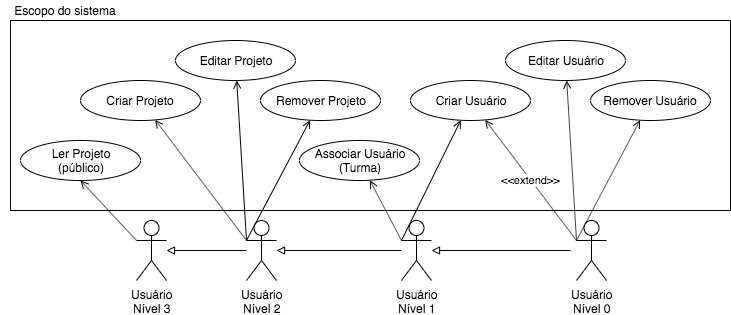
\includegraphics[width=1.0\hsize]{figuras/diag_use_case.png}
  \legend{Nível 0: Administrador; Nível 1: Professor; Nível 2: Aluno; Nível 3: Visitante (Anônimo).}
  \source{A autora, 2018.}
\end{figure}

O digrama tem como função mapear as interações previstas dos atores do LFSR com o banco de dados. A documentação gerada pelo mesmo se encontra no apêndice \ref{ap2}. Como as restrições a serem aplicadas dependem de comandos SQL do tipo DCL(\textit{Data Control Language}), o código de implementação do projeto piloto não incluíram os requisitos modelados neste diagrama de caso de uso. Isto significa que este requisito foi levantado, mapeado, porém não implementado.

Da análise imediata dos requisitos são identificadas duas entidades sobre as quais irão operar as funcionalidades registradas como requisitos. São o ``usuário do LFSR'' e o ``projeto fotogramétrico''. Por simplificação, as seções seguintes irão adotar convenções como, por exemplo, ``requisitos de projeto'' para referir-se às funções de inserção, recuperação, atualização e, em alguns casos, remoção, da entidade ``projeto'' fotogramétrico, ou seja, neste trabalho está sendo simplificado ``requisitos de pertinência do projeto fotogramétrico'' para a primeira forma apresentada. Demais requisitos de associação das entidades ou imposição de regras serão nomeados diretamente, sem simplificação, quando necessário.


\subsection{Identificação das Entidades Principais do Acervo} \label{entidades}

Logo de início, foi questionado \textit{``quais dados comporiam o acervo?''}. A resposta levou à identificação dos tipos de dados encontrados no acervo, compostos em sua grande maioria, por imagens em formato analógico (fotogramas). Foram encontrados, também, alguns registros de projetos de alunos antigos ou projetos disponibilizados ao LFSR, registros de pontos e dados relacionados a sensores, não necessariamente vinculados aos projetos fotogramétricos.

O software e-foto, como parte fundamental do LFSR, tem capacidade de trabalhar com outros projetos fotogramétricos fora os disponibilizados atualmente em seu \textit{website}. O próprio laboratório possui total capacidade de trabalhar com outros projetos, sejam eles fotogramétricos ou de sensoriamento remoto. Isso leva ao segundo questionamento \textit{``de que formas esse dados poderiam ser expandidos?''}. Para o qual registra-se no contexto deste trabalho que atualmente, o conjunto de dados não é mais composto só pela realidade atual do acervo do LFSR, mas também de uma previsão da realidade futura. Dessa forma, ao responder tal questionamento foi possível prever, em parte, a criação de uma solução que, em pouco tempo, poderia se tornar obsoleta. Nesta hipótese, o conjunto de dados previsto engloba o acervo e os dados relacionados a um projeto aerofotogramétrico tradicional e estima-se a necessidade de extensão contínua do modelo, enquanto houverem evoluções do conjunto de dados do acervo.

Os requisitos principais e por consequência a entidade principal é identificada quando o objetivo da fotogrametria é definido como ``a reconstrução de um espaço tridimensional, chamado de espaço-objeto, a partir de um conjunto \textbf{não vazio de imagens bidimensionais}, chamado de espaço-imagem'' \cite[p.16]{coelho2007fotogrametria}. Assim fica claro que a entidade fundamental dentre aquelas que mapeiam o acervo para o laboratório de fotogrametria é a \textbf{imagem}. 

Para auxiliar a identificação de outras entidades principais fez-se uso do fluxo de trabalho do projeto E-Foto. A partir dele foram destacadas as atividades da fase de Inicialização do Projeto, descrito na seção \ref{efoto}, que apresenta o fluxo de trabalho fotogramétrico. Os dados de \textbf{projeto}, como \textbf{voo} e \textbf{sensor}, são atribuídos na atividade de Criação e Gerenciamento do Projeto Fotogramétrico. Na atividade seguinte, Aquisição e Cadastro de Dados são fornecidos informações a respeito das \textbf{imagem} e dos \textbf{pontos}, adquiridos nos levantamentos aéreo e terrestre, respectivamente. Orientação Interior e Orientação Exterior são atividades de processamento, e, enquanto importantes, ambas geram parâmetros relacionados à imagem e, por tanto, caracterizam a presença de entidades fracas. Por último, as fases de Geração de produtos e Integração, que envolvem o processamento e distribuição dos \textbf{produtos} finais da fotogrametria, ficaram fora do escopo deste trabalho. A relação entre as entidades principais identificadas podem ser ilustrados como na figura \ref{requisitos}.

\begin{figure}[!ht]{13cm}
  \caption{Identificação das entidades principais pela análise de requisitos} \label{requisitos}
  \centering
  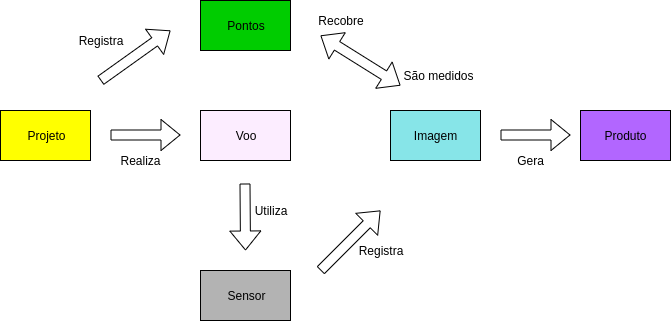
\includegraphics[width=1.0\hsize]{figuras/diagrama_requisitos.png}
  %\legend{Texto da legenda quando necessário.}
  \source{A autora, 2018.}
\end{figure}

Todo o projeto fotogramétrico, como comentado no item \ref{efoto}, é responsável pelo armazenamento de metadados relativos ao processo fotogramétrico. É nele que dados como: responsável pelo projeto; criação e data de modificação etc, são armazenados. 
Voltando aos itens \ref{sensor_img} e \ref{foto_trad}, para todo levantamento aéreo, com finalidade fotogramétrica, é indispensável a presença do sensor imageador na aeronave, pois o mesmo é responsável pela aquisição das imagens.
Segundo \citeonline[p.32-39]{projeto1999dalmolin} pontos de controle ou apoio devem ser demarcados na região fotografada, podendo ser medidos antes do levantamento aéreo ou depois. Os projetos fotogramétricos podem depender ainda de pontos fotogramétricos, cujas coordenadas no espaço objeto só serão determinadas ao final da fase de inicialização fotogramétrica. Porém, o autor deixa claro que os pontos, independentemente do tipo ou finalidade, devem ser visíveis nas fotografias, de modo a serem utilizados no projeto.
Por fim, percebe-se na obra de \citeonline{coelho2007fotogrametria}, que diversos produtos são gerados a partir do processo fotogramétrico. Sabendo que, nesses processos, a imagem pode ser considerada como dado central, fica fácil perceber que o produto fotogramétrico é gerado, independentemente do método, a partir das imagens cadastradas.

Assumindo que esses são os principais requisitos de persistência e estão associados à entidades fortes, foi adotado que para cada entidade principal existe um pacote de mesmo nome. Cada pacote deve receber o nome de suas respectivas entidades principais e conter demais entidades diretamente relacionadas às principais.

Nesse momento, o próximo passo foi questionar: \textit{``exitem normas que identifiquem e padronizem essas entidades?''}, \textit{``caso essas normas existam, elas atendem os objetivos estabelecidos neste trabalho?''}. Tentando responder a essas perguntas, chegou-se ao Perfil de Metadados Geográficos do Brasil \cite{pmgb2009}. Porém o mesmo, como o próprio nome diz, trata de metadados e inclui imagem como tal, entrando em conflito com a expectativa da fotogrametria, que considera a imagem seu dado principal.

A questão anterior foi também analisada no âmbito internacional. À primeira vista, a padronização esperada foi pesquisada na documentação da OGC, mas como estava baseada nas normas de padronização ISO o que implicou na necessidade de se consultar as mesmas. Neste momento foram encontrados muitos obstáculos. Como, por exemplo, o custo de aquisição da ISO, que limita o acesso às mesmas, restringindo à parte da documentação disponível ao acesso público. Dentre as ISO pesquisadas foi constatado que enquanto algumas atendiam parte das entidades esperadas para alguns pacotes, todas se desdobravam em outras ISO, ao ponto em que a documentação necessária pra a criação do modelo seria demasiadamente extensa. Assim, ao se tentar utilizar todas as ISO, necessárias para criação de parte do modelo, se acabaria por ter um novo padrão, o que foge ao objetivo inicial.

Ao considerar todos esses fatores, observou-se que não foi encontrado uma norma, ou conjunto de normas que atendesse o projeto. Assim, partiu-se para a identificação das outras entidades envolvidas em um processo fotogramétrico com a seguinte pergunta \textit{``quais entidades complementam as já identificadas e como elas se comunicam?''}. No item \ref{model} é descrito como foi realizada a modelagem da comunicação entre as entidades. Porém, antes desse modelo ser criado, deve-se responder a primeira parte dessa pergunta e identificar os requisitos faltantes para complementar um processo fotogramétrico.  

\citeonline[p.1-6]{projeto1999dalmolin} define três fases a serem realizadas durante o planejamento de projeto fotogramétrico com fotografias aéreas. As duas primeiras fases resumem, em poucas palavras, boa parte das entidades e onde elas se encontram no processo fotogramétrico:

 \begin{itemize}
     \item Planejamento de voo leva em consideração as informações relativas ao terreno. As informações do sensor, usadas junto com os dados do terreno, permitem ao técnico definir linhas de voo, porcentagem de sobreposição entre as fotografias tomadas, quantidade final de fotografias tomadas, direção de voo etc.
     \item Planejamento do controle de terreno e execução dos levantamentos de campo. Estes geram os pontos que são medidas nas imagens.
 \end{itemize}

Analisando o planejamento de voo, identifica-se a existências de dados relativos ao \textbf{voo}, ao \textbf{terreno}, ao \textbf{sensor}, ao rodapé da imagem, que nada mais é do que à projeção, no terreno, das fotografias tomadas sobre o terreno e as próprias \textbf{imagens}. O sensor, por sua vez, define a \textbf{geometria} da fotografia tirada, sendo o \textit{frame} (quadro) o caso mais comum. Na segunda fase são identificados os \textbf{pontos}, que podem ser obtidos através do \textbf{levantamento} topográfico. Esses pontos formam \textbf{coleções} associadas pelo levantamento à região geográfica em que se encontram.

\citeonline[p.89]{coelho2007fotogrametria} comentam que para que sejam possíveis as medições de coordenadas no espaço-imagem, as imagens do voo acabam por ser `orientadas'. Ou seja, os parâmetros das orientações interior e exterior devem ser incorporados às imagens durante o processo fotogramétrico. O processo de fototriangulação é o principal meio de computação dos parâmetros de orientação, contudo processos para imagens isoladas podem ser executados como alternativa, a exemplo do processo de ressecção espacial. Este fato em junção da previsão do modelo poder abranger outros processos levam à caracterização dos \textbf{parâmetros} como entidades agregadas (entidades fracas), que se relacionam às imagens e a um modelo paramétrico adotado no projeto, para descrever o sistema de equações adotadas no projeto. Estima-se que tais indicações podem auxiliar na fixação do modelo para futuras entradas de dados de outros processos como ocorreria na implementação do uso de imagens provenientes de satélite que geralmente são acompanhadas de RPCs.

Vale ressaltar que nem todos o requisitos de persistência identificados geraram entidades fortes no modelo conceitual. Consequentemente algumas entidades vão surgir durante a especificação do modelo que antecede a implementação. Por exemplo, a representação de \textbf{rodapé} necessita de um maior detalhamento para que sua entidade possa ter uma especificação como classe e a devida associada com a entidade imagem mapeada. Rodapé da imagem, como visto na figura \ref{foot}, refere-se à região de cobertura no terreno associada à respectiva imagem. Isso significa que nem todo termo fotogramétrico está elicitado nos requisitos levantados para as primeiras versões do modelo e torna evidente a necessidade de um modelo de desenvolvimento ágil. Por fim, a adição deste requisito, implica na possibilidade de adição de diversas entidades no modelo como faixa e par que não eram bem estruturados até a integração do conceito de rodapé.

\begin{figure}[!ht]{10cm}
  \caption{Exemplo de rodapé de imagens.} \label{foot}
  \centering
  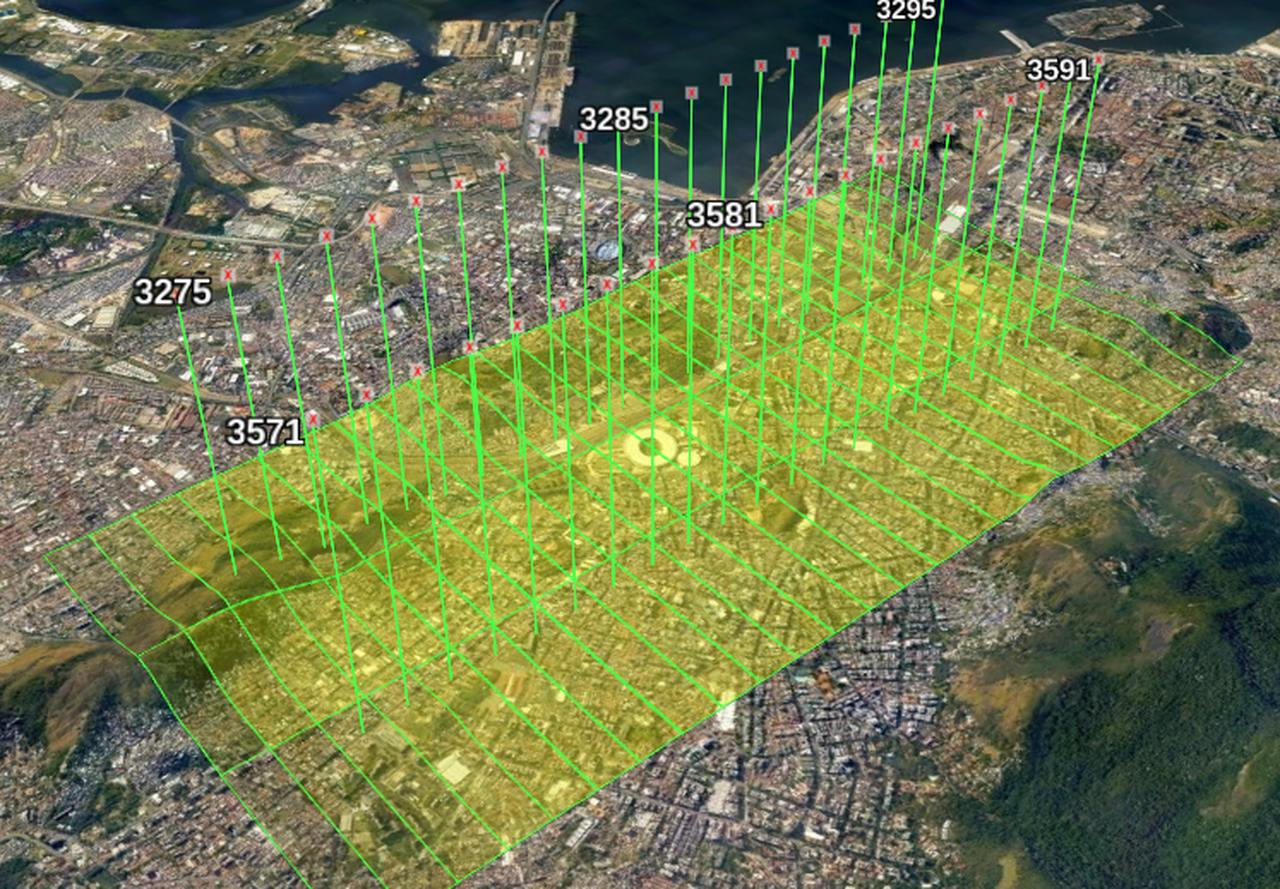
\includegraphics[width=1\hsize]{figuras/footprint.jpg}
  \legend{Imagem adaptada pela autora no software Google Earth Pro, utilizando os dados de levantamento aéreo sobre o Rio de Janeiro no de 2003 realizado pelo IPP}
  \source{A autora, 2019.}
\end{figure}

Como comentado no item \ref{foto_trad}, existe uma sobreposição de imagens acarretando em, no mínimo, a existência de um ``par de imagens''. Esse par de imagens são necessários para ocorrer a estereoscopia. Várias imagens tomadas em sequência formam uma ``faixa''. O grupo de faixas de um mesmo voo podem formar um ``bloco''.

As entidades destacadas até então podem ser subdivididas em três categorias: (1) entidades principais; (2) entidades complementares; e (3) entidades derivadas. Entidades complementares são entidades internas aos pacote para completude ou associatividade do modelo, tendo como dados de entrada, dados brutos ou dados de associação dos elementos presentes no acervo ao projeto fotogramétrico. Já as entidades de dados derivados armazenam dados obtidos através de cálculos. A tabela \ref{entidades_cat} mostra um exemplo de distribuição das entidades analisadas em suas respectivas categorias.

\begin{table}[!ht]{14cm}
  \caption{Exemplos de entidades separadas por categorias.}\label{entidades_cat}
    \begin{tabular}{ccc}
    \hline
    \rowcolor[HTML]{333333} 
    {\color[HTML]{FFFFFF} \textbf{Principal}} & {\color[HTML]{FFFFFF} \textbf{Complementar}} & {\color[HTML]{FFFFFF} \textbf{Derivadas}} \\ \hline
    \rowcolor[HTML]{EFEFEF} 
    \begin{tabular}[c]{@{}c@{}}Projeto\end{tabular} & \begin{tabular}[c]{@{}c@{}}Terreno\end{tabular} & \begin{tabular}[c]{@{}c@{}}Parâmetros\end{tabular} \\
    
    \begin{tabular}[c]{@{}c@{}}Ponto\end{tabular} & \begin{tabular}[c]{@{}c@{}}Levantamento do terreno\end{tabular} & \begin{tabular}[c]{@{}c@{}}\textit{Rodapé}\end{tabular} \\
    
    \rowcolor[HTML]{EFEFEF} 
    \begin{tabular}[c]{@{}c@{}}Sensor\end{tabular} & \begin{tabular}[c]{@{}c@{}}Especificações do sensor\end{tabular} & \begin{tabular}[c]{@{}c@{}}Produtos\end{tabular} \\
    
    \begin{tabular}[c]{@{}c@{}}Voo\end{tabular} & \begin{tabular}[c]{@{}c@{}}Bloco\end{tabular} & \begin{tabular}[c]{@{}c@{}}\end{tabular} \\
    
    \rowcolor[HTML]{EFEFEF} 
    \begin{tabular}[c]{@{}c@{}}Imagem\end{tabular} & \begin{tabular}[c]{@{}c@{}}Faixa\end{tabular} & \begin{tabular}[c]{@{}c@{}} \end{tabular} \\
    
    \begin{tabular}[c]{@{}c@{}}\end{tabular} & \begin{tabular}[c]{@{}c@{}}Par\end{tabular} & \begin{tabular}[c]{@{}c@{}}\end{tabular} \\ 
    %\rowcolor[HTML]{EFEFEF} 
    %\begin{tabular}[c]{@{}c@{}}\end{tabular} & %\begin{tabular}[c]{@{}c@{}}\end{tabular} &
    %\begin{tabular}[c]{@{}c@{}}\end{tabular} \\
    \hline
    \end{tabular}
  \source{A autora, 2019}
\end{table}



\section{Modelagem}\label{model}

Após o levantamento e análise de requisitos, o passo seguinte foi de modelagem. Este consistiu na construção de diagramas para especificar as classes que permitissem a representação das entidades a serem persistidas no banco, levando em consideração suas conexões e possíveis agrupamentos em pacotes. Como explicado no item \ref{mod_bd}, a modelagem adotada deve suportar dados alfanuméricos e geográficos. A linguagem escolhida foi a UML 2.0 e a especificação de classes e tipos de dados está inclusa nos apêndices deste trabalho. A seguir, serão apresentadas as justificativas e tomadas de decisão que levaram ao conjunto de classes modeladas, com dicionários de dados para estas classes e os diagramas de pacotes.


\subsection{Modelo Orientado a Objetos}

O modelo idealizado para o LFSR tem sua nomenclatura escrita em inglês. Essa decisão foi tomada em função da internacionalização do projeto E-Foto. Como este, por sua vez, serviu de base para muitas partes do modelo desenvolvido neste trabalho, optou-se por seguir este padrão para nomenclatura. O que torna o modelo em construção aderente aos trabalhos anteriores que foram desenvolvidos no projeto E-Foto. Para o modelo ser elaborado foi necessário conhecer todos os detalhes de um projeto fotogramétrico. O conhecimento se baseia na leitura de diferentes autores e obras, todos presentes na bibliografia deste trabalho.

Muitos autores começam explicando o mapeamento fotogramétrico pelo plano de voo, indicando que o planejamento deve ser a primeira atividade a ser feita. Enquanto essa concepção não está errada, ao se planejar um voo o projeto fotogramétrico é iniciado. Por se tratar da modelagem de um banco de dados, deve-se considerar os metadados do mapeamento fotogramétrico. Isso significa que o primeiro objeto a ser modelado é a classe \textit{Project}:

\begin{description}[labelwidth=2cm, itemsep=-0.3cm]
    \item [Classe Project]
    \item [Id:] Índice numérico;
    \item [Name:] Nome do projeto;
    \item [Owner:] Responsável, ou dono, do projeto;
    \item [Date\_add:] Data de criação do projeto no banco;
    \item [Date\_mod:] Última data de modificação do projeto;
    \item [Software:] Programa computacional responsável pelo processamento de dados;
    \item [Id\_srs:] Referência para a classe \textit{Srs}.
\end{description}

A figura \ref{project}, no apêndice \ref{ap0}, resume os atributos da classe \textit{Project} e os tipos de dados adotados durante sua implementação.

Qualquer projeto armazenado no banco, por conter a dados geográficos, deve possuir projeção cartográfica, sistema de referência geodésico e quaisquer dados complementares destes primeiros. É importante saber quais são os referenciais e projeções aplicáveis para proceder transformações de compatibilização nos dados de entrada e saída para cada projeto. A classe \textit{Srs} é responsável por armazenar esses dados:

\begin{description}[labelwidth=2cm, itemsep=-0.3cm]
\item [Classe Srs]
\item [Id:] Índice numérico;
\item [Epsg:] Referência ao  campo `srid' na tabela `spatial\_ref\_sys', comum nos SGBDs espaciais.
\end{description}

O EPSG é um vantagem presente em algumas extensões de bancos de dados espaciais. O Grupo de Pesquisa Petrolífera Européia ( \textit{European Petroleum Survey Group} - EPSG) é responsável pela criação dos `Códigos EPSG'. Informalmente conhecidos como simplesmente EPSG, essa lista de valores numéricos é uma combinação que serve de índice para sistemas de referência de coordenadas em todo o planeta.

As coordenadas do ponto central da região geográfica de trabalho, também são associadas a um projeto fotogramétrico. Tal dado se justifica em função da correção do efeito sistemático da curvatura da Terra no cálculo da aerotriangulação, onde é utilizado o método de ajustamentos de um bloco de imagens por feixes perspectivos. Esse efeito é notável em escalas médias e pequenas, isto é, menores ou iguais à 1:30.000, sendo geralmente negligenciado para escalas cadastrais (1:10.000 e maiores). A classe \textit{Cg\_central\_area} inclui tais informações.

\begin{description}[labelwidth=2cm, itemsep=-0.3cm]
\item [Classe Cg\_central\_area]
\item[Id\_proj:] Referência para a classe \textit{Project};
\item[Proj\_ctr:] Coordenadas planimétricas do centro da região de interesse do projeto.
\end{description}

Estas três classes compõem o pacote \textbf{Project}. A figura \ref{pack_proj} ilustra como essas classes se comunicam entre si, e com outros pacotes.

\begin{figure}[!ht]{13cm}
  \caption{Pacote Project} \label{pack_proj}
  \centering
  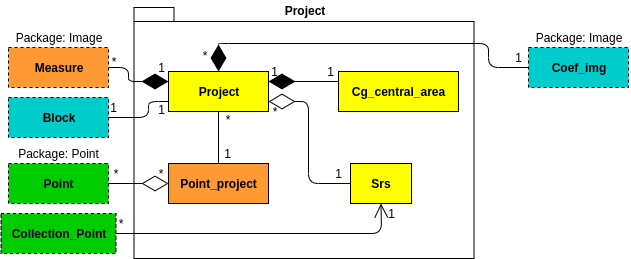
\includegraphics[width=1\hsize]{figuras/package_proj.png}
  %\legend{Texto da legenda quando necessário.}
  \source{A autora, 2019.}
\end{figure}

Definido o projeto pode-se partir para o levantamento aéreo. No planejamento de voo, dados do terreno da região a ser sobrevoada são coletados. Estes devem ser armazenados na classe \textit{Terrain}.

\begin{description}[labelwidth=2cm, itemsep=-0.3cm]
\item [Classe Terrain]
\item[Id:] Índice numérico;
\item[Alt\_max:] Valor da altitude máxima do terreno em metros;
\item[Alt\_min:] Valor da altitude mínima do terreno em metros;
\item[Alt\_med:] Valor da altitude média do terreno em metros.
\end{description}

A classe \textit{Flight} é responsável pela armazenagem de dados relativos ao aerolevantamento. Além das informações que permitem identificar o voo, esta classe deve preservar a associação com o sensor usado e o terreno levantado. Adota-se a generalização de levantamento (\textit{survey}) para os projetos que fornecem insumos para os projetos fotogramétricos, pois estes ter seus dados reaproveitados total ou parcialmente em diferentes projetos de fotogrametria.

\begin{description}[labelwidth=2cm, itemsep=-0.3cm]
\item [Classe Flight]
\item[Id:] Índice numérico;
\item[Date:] Data de execução do aerolevantamento;
\item[Num\_ser:] Número de série do aerolevantamento;
\item[Num\_auth:] Número de autorização do aerolevantamento;
\item[Id\_sensor:] Referência para a classe \textit{Sensor};
\item[Id\_terrain:] Referência para a classe \textit{Terrain};
\item[Id\_survey:] Referência para a classe \textit{Survey}.
\end{description}

Existem dados complementares ao voo que são essenciais para o projeto fotogramétrico. Tais dados estão isolados na classe \textit{Param\_flight}.
Eles incluem a sobreposição entre fotogramas adjacentes, ao longo de uma faixa de voo, denominada de ``sobreposição longitudinal'' e a sobreposição entre faixas de voos adjacentes caracterizando a ``sobreposição lateral''. Essas sobreposições visam assegurar a estereoscopia em toda a área a ser mapeada.
Além destes, tem-se a altitude em relação ao nível dos mares e a escala nominal do voo, com a qual se sabe qual é a resolução espacial do terreno no mapa de interesse. Sendo que esta, por sua vez, é obtida pela relação entre a focal da câmera e altura de voo.

\begin{equation} \label{escala}
   E = \frac{f}{H}
\end{equation}

Onde:

E: Escala nominal ou média do voo;

f: Distância focal da câmara;

H: Altura do voo em relação ao plano médio do terreno.

\begin{description}[labelwidth=2cm, itemsep=-0.3cm]
\item [Classe Param\_flight]
\item[Id:] Índice numérico;
\item[Id\_flight:] Referência para a classe \textit{Flight};
\item[Alt\_sea\_lvl:] Altitude em relação ao nível do mar, em metros;
\item[Den\_scale:] Denominador da escala nominal;
\item[Overlap\_l:] Sobreposição entre fotos;
\item[Overlap\_s:] Sobreposição entre faixas.
\end{description}

A classe \textit{bounding\_box} é responsável pelo armazenamento das coordenadas dos vértices da diagonal de um retângulo imaginário que recobre toda a região fotografada. O software e-foto, apesar de ainda não trabalhar com tal dado, pode vir a contemplar essa informação. Este dado foi adicionado ao modelo, pois ele permite a realização várias atividades. Com ele, é possível por exemplo, realizar observações de erros grosseiros em pontos do projeto. Tal classe pode permitir a composição de um retângulo envolvente partindo de dois vértices, operação normalmente suportada pelos SGBDs com extensão espacial.

\begin{description}[labelwidth=2cm, itemsep=-0.3cm]
\item [Classe Bouding\_box]
\item[Id:] Índice numérico;
\item[Xy\_ul:] Coordenadas do vértice superior esquerdo;
\item[Xy\_br:] Coordenadas do vértice inferior direito;
\item[Id\_terrain:] Referência para a classe \textit{Terrain};
\item[Id\_flight:] Referência para a classe \textit{Flight}.
\end{description}

As interações entre as classes do pacote \textbf{Flight} e as classes de outros pacotes é ilustrada na figura \ref{pack_fli}.

\begin{figure}[!ht]{13cm}
  \caption{Pacote Flight} \label{pack_fli}
  \centering
  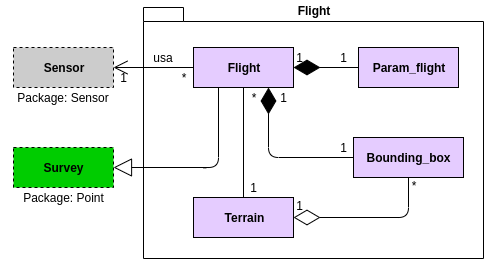
\includegraphics[width=1\hsize]{figuras/package_voo.png}
  %\legend{Texto da legenda quando necessário.}
  \source{A autora, 2019.}
\end{figure}

Neste modelo se adota o uso de um sensor para cada voo. A possibilidade de serem armazenados múltiplos sensores por voo pode ser adotada em uma extensão do modelo conceitual à ser realizada em trabalhos futuros. 

Os metadados desse sensor são armazenados no pacote \textbf{Sensor}, ilustrado na figura \ref{pack_sen}. Tem-se os dados do sensor conectados pela classe \textit{sensor}.

\begin{description}[labelwidth=2cm, itemsep=-0.3cm]
\item [Classe Sensor]
\item[Id:] Índice numérico;
\item[Id\_spec:] Referência para a classe \textit{Specification}; 
\item[Desc:] Descrição que o usuário pode usar para diferenciar seus sensores. 
\end{description}

Cada sensor possui especificações atreladas.  A classe \textit{Specification} contém essas informações. Note-se que as especificações de diversos sensores podem ser iguais se forem adotados equipamentos distintos de um mesmo modelo e fabricante. Tais valores são comuns aos diferentes equipamentos. Pequenas variações detectáveis em processos de calibração serão isolados em outra classe.

\begin{description}[labelwidth=2cm, itemsep=-0.3cm]
\item [Classe Specification]
\item[Id:] Índice numérico;
\item[Brand:] Modelo do sensor; 
\item[Manufact:] Fabricante do sensor;
\item[Focal:] Distância focal nominal da câmara em mm;
\item[Pixel\_size:] Tamanho do pixel no sensor; 
\item[Rows:] Quantidade de linhas do sensor;
\item[Cols:] Quantidade de colunas do sensor;
\item[Detector:] Identificador do tipo de sensor;
\end{description}

O atributo `\textit{Detector}' define se as imagens geradas pelo sensor serão de origem digital, ou analógica. Para tanto foi criado um \textit{data type}, ilustrado pela figura \ref{typesensor} do apêndice \ref{ap0}, que permite o armazenamento no banco justamente destes tipo enumerado.

Devido as pequenas variações a que estão submetidos os parâmetros internos do sensor por questões construtivas ou devido ao estresse de operação, não se recomenda a execução do processamento fotogramétrico sem os dados presentes no certificado de calibração. Tais dados podem ainda variar ao longo do tempo, motivo pelo qual uma data de validade de vinculada. Isto transmite a noção de que um mesmo sensor poderá ter diferentes calibrações, configurando a composição ``um para muitos'' entre a classe \textit{Sensor} e a classe \textit{Calibration} expressa a seguir. 

\begin{description}[labelwidth=2cm, itemsep=-0.3cm]
\item [Classe Calibration]
\item[Id:] Índice numérico;
\item[Id\_sensor:] Referência para a classe \textit{Sensor};
\item[Date\_cria:] Data de criação; 
\item[Date\_end:] Data de expiração;
\item[Number:] Número de série do certificado;
\item[Focal\_clb:] Focal calibrada da câmara em mm; 
\item[S\_focal\_clb:] Desvio-padrão da focal calibrada;
\item[Ppx:] Coordenada X do ponto principal do sensor em mm;
\item[Ppy:] Coordenada Y do ponto principal do sensor em mm;
\item[S\_ppx:] Desvio-padrão da coordenada X do ponto principal do sensor;
\item[S\_ppy:] Desvio-padrão da coordenada Y do ponto principal do sensor;
\item[Id\_sym:] Referência para classe \textit{Symmetric\_distortion};
\item[Id\_dec:] Referência para a classe \textit{Decentering\_distortion}.
\end{description}

Como o acervo comporta inúmeras imagens de origem analógica, as propriedades de câmaras métrica de formato analógico devem ser suportadas. Isso implica no registro de informações sobre as marcas fiduciais que são normalmente conferidas no processo de calibração. Por tanto, é esperado que a classe \textit{ficucials} represente um conjunto de informações que servirá apenas para vincular informações dos sensores analógicos.

\begin{description}[labelwidth=2cm, itemsep=-0.3cm]
\item [Classe Fiducials]
\item[Id:] Índice numérico;
\item[Id\_calib:] Referência para a classe \textit{Calibration};
\item[X:] Coordenada X em mm;
\item[Y:] Coordenada Y em mm; 
\item[Sigma\_x:] Desvio-padrão da coordena X;
\item[Sigma\_y:] Desvio-padrão da coordenada Y.
\end{description}

Ao capturar uma imagem, o feixe de luz pode sofrer desvios (como visto no item \ref{sensofot}). Duas das distorções que afetam a posição dos objetos imageados, são chamadas de radial simétrica e descentrada. Soluções matemáticas, dadas pelos sistemas de equações \ref{sim1} e \ref{des1}, ambos precisam de dados que são informados no certificado de calibração. As classes \textit{Symmetric\_distortion} e  \textit{Decentering\_distortion} conectam esse dados ao certificado de calibração. 

O modelo adotado para a distorção radial simétrica é: 

\begin{equation} \label{sim1}
\begin{array}{cl}
\delta x &= (k0 + k1r^{2} +k2r^{4} +k3r^{6})x" \\
\delta y &= (k0 + k1r^{2} +k2r^{4} +k3r^{6})y" \\
x' &= x'' - \delta x \\
y' &= y'' - \delta y
\end{array}
\end{equation}

Onde:

$\delta$x, $\delta$y: componentes da distorção radial simétrica;

r é o raio a partir do ponto principal de simetria;

k0, k1, k2, k3: coeficientes do certificado de
calibração;

x”, y”: coordenadas do ponto sem correção, referidas ao ponto principal de simetria;

x’, y’: as coordenadas corrigidas da distorção radial simétrica.

\begin{description}[labelwidth=2cm, itemsep=-0.3cm]
\item [Classe Symmetric\_distortion]
\item[Id:] Índice numérico;
\item[Id\_calib:] Chave estrangeira que faz referência ao atributo `Id' da classe `Calibration';
\item[K0:] Coeficiente k0 de distorção da lente;
\item[K1:] Coeficiente k1 de distorção da lente;
\item[K2:] Coeficiente k2 de distorção da lente;
\item[K3:] Coeficiente k3 de distorção da lente; 
\item[Sigma\_k0:] Desvio-padrão do coeficiente k0;
\item[Sigma\_k1:] Desvio-padrão do coeficiente k1;
\item[Sigma\_k2:] Desvio-padrão do coeficiente k2;
\item[Sigma\_k3:] Desvio-padrão do coeficiente k3.
\end{description}

A distorção descentrada é resolvida, por sua vez, adota as formulações: 

\begin{equation} \label{des1}
\begin{array}{cl}
\delta x' &= p1(r^{2}+x"^{2})+p2r^{2}x"^{2}y"^{2} \\
\delta y' &= p1(r^{2}+y"^{2})+p2r^{2}x"^{2}y"^{2} \\ 
x &= x' - \delta x'\\
y &= y' - \delta y'
\end{array}
\end{equation}

Onde:

$\delta$x', $\delta$y': componentes da distorção radial descentrada;

r é o raio a partir do ponto principal de simetria;

p1, p2: coeficientes do certificado de calibração;

x”, y”: coordenadas do ponto sem correção, referidas ao ponto principal de simetria;

x’, y’: coordenadas corrigidas da distorção radial descentrada;

x, y: coordenadas corrigidas das duas distorções.

\begin{description}[labelwidth=2cm, itemsep=-0.3cm]
\item [Classe Decentering\_distortion]
\item[Id:] Índice numérico;
\item[P1:] Coeficiente P1 de distorção da lente;
\item[P2:] Coeficiente P2 de distorção da lente; 
\item[Sigma\_p1:] Desvio-padrão do coeficiente p1;
\item[Sigma\_p2:] Desvio-padrão do coeficiente p2.
\end{description}

\begin{figure}[!ht]{13cm}
  \caption{Pacote Sensor} \label{pack_sen}
  \centering
  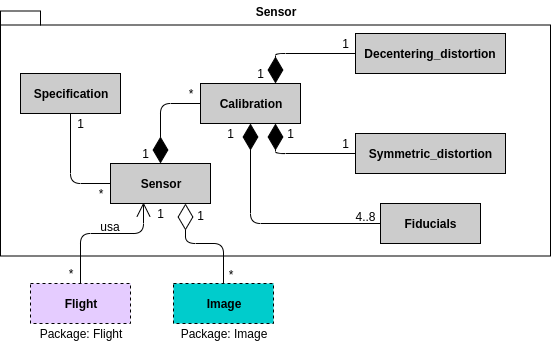
\includegraphics[width=1\hsize]{figuras/package_sensor.png}
  %\legend{Texto da legenda quando necessário.}
  \source{A autora, 2019.}
\end{figure}

Na etapa `Aquisição e Cadastro de Dados' do item \ref{efoto} se gerados os dados dos pacotes \textbf{Image} e \textbf{Point}. Como algumas classes de imagem mencionam algumas informações pertencentes às classes de pontos, decidiu-se apresentar o último antes do primeiro, evitando assim que houvesse a necessidade da quebra da imagem na apresentação adotada neste trabalho para tal pacote. Isso é dito pois, o levantamento topográfico normalmente é feito depois da captação das fotografias aéreas.

\textit{Point} é a classe principal do pacote de mesmo nome. A obtenção de seus dados são a razão pelo qual um levantamento topográfico é realizado. Esta classe possui dados geográficos. Por tanto pode ser usada com um exemplo claro da presença de dados complexos no modelo e a necessidade de trabalhar com um banco que possua extensões para dados geográficos. Adotar tal recurso permite indexação e consequente aceleração nas buscas por pontos numa dada região de interesse quando isto for de interesse dos usuários do banco de dados sob desenvolvimento.

%Figura \ref{point}: \textbf{Classe Point}
\begin{description}[labelwidth=2cm, itemsep=-0.3cm]
\item [Classe Point]
\item[Id:] Índice numérico;
\item[Name:] Nome do ponto;
\item[Geom:] Coordenadas tridimensionais do ponto (pointz);
\item[Sigma:] Desvio-padrão das coordenadas do ponto;
\item[Id\_coll:] Referência para a classe \textit{Collection}.
\end{description}

Vários pontos formam uma coleção de pontos. Um levantamento topográfico pode ser feito em dias distintos, ou seja, podem possuir várias coleções de pontos. Ao mesmo tempo, um projeto fotogramétrico pode selecionar subconjuntos de pontos nas diferentes coleções disponíveis de levantamentos topográficos na região de interesse do projeto fotogramétrico. Estas associações requerem tabelas de associação e para explicitá-las foram estipuladas as classes de ligação \textit{Collection\_point} e \textit{Point\_project} respectivamente.

\begin{description}[labelwidth=2cm, itemsep=-0.3cm]
\item [Classe Collection\_Point]
\item[Id:] Índice numérico;
\item[Id\_srs:] Referência para a classe \textit{Srs};
\item[Date:] Data da coleta da coleção de pontos;
\item[Receptor:] Receptor da antena;
\item[Antenna:] Antena usada no levantamento;
\item[Ant\_lvl:] Altura da antena em m;
\item[Id\_survey:] Referência para a classe \textit{Ground\_survey}.
\end{description}

É importante notar que esta classe tem uma coloração diferente do resto no pacote. Este destaque foi usado para destacar a entidade associativa que liga duas classes principais e, por consequência, dois pacotes.  

\begin{description}[labelwidth=2cm, itemsep=-0.3cm]
\item [Classe Point\_project]
\item[Id\_proj:] Referência para a classe \textit{Project};
\item[Id\_point:] Referência para a classe \textit{point};
\item[Use:] Função que o ponto está exercendo no projeto fotogramétrico.
\end{description}

O mesmo ponto pode ser de controle, fotogramétrico ou usado como ponto de verificação. Seu uso varia de acordo com o projeto que se esta trabalhando. Para definir esse uso, foi criado um \textit{data type} específico, apresentado na figura \ref{pointype} do apêndice \ref{ap0}.

Por último, na classe \textit{Ground\_survey} do pacote \textbf{Point}, representado na figura \ref{pack_point}, se encontram os metadados do levantamento topográfico. 

\begin{description}[labelwidth=2cm, itemsep=-0.3cm]
\item [Classe Ground\_survey]
\item[Id:] Índice numérico;
\item[Id\_Survey:] Referência para a classe \textit{Survey};
\end{description}

\begin{figure}[!ht]{13cm}
  \caption{Pacote Point} \label{pack_point}
  \centering
  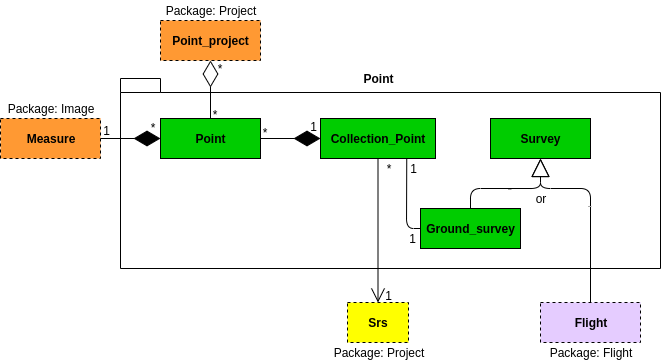
\includegraphics[width=1\hsize]{figuras/package_point.png}
  %\legend{Texto da legenda quando necessário.}
  \source{A autora, 2019}
\end{figure}

O último pacote a ser apresentado é o pacote \textbf{Image}. Foram modelados e implementados, até o momento da defesa deste trabalho, os dados relacionados às imagens geradas a partir de um aerolevantamento. O uso de fotos analógicas deve prever a digitalização deste materiais para permitir o processamento digital pelas ferramentas de software disponíveis no LFSR.

Marcas fiduciais, nas fotos de câmaras métricas, bem como, pontos no terreno são associados as imagens através do processo de medição. Assim obtém-se para cada ponto existente no terreno (espaço-objeto) um conjunto de medidas análogas (no espaço-imagem), em \textit{pixels}. A classe \textit{measure} realiza a analogia entre tais sistemas de coordenadas.

\begin{description}[labelwidth=2cm, itemsep=-0.3cm]
\item [Classe Measure]
\item[Row:] Número da linha em que se encontra o pixel;
\item[Col:] Número da linha em que se encontra o pixel;
\item[Id\_img:] Referência para a classe \textit{Image};
\item[Id\_point:] Referência para a classe \textit{Point};
\item[Id\_proj:] Referência para a classe \textit{Project}.
\end{description}

A classe principal deste pacote é a classe \textit{image} que contém os metadados do fotograma digitalizado ou da fotografia digital. 

\begin{description}[labelwidth=2cm, itemsep=-0.3cm]
\item [Classe Image]
\item[Id:] Índice numérico;
\item[Name:] Nome da imagem;
\item[Resolution:] Resolução da imagem;
\item[Size\_pixels:] Resolução da imagem em numero de linhas e colunas de pixels;
\item[Img\_type:]  Define o tipo de imagem armazenada (para diferenciar ortoimagens em extensões);
\item[Id\_sensor:]  Referência para a classe \textit{Sensor};
\item[Id\_strip:] Referência para a classe \textit{Strip}.
\end{description}

Como se trata de um modelo de banco de dados voltado para o acervo de um laboratório, um dos dados mais importantes é a armazenagem dos arquivos digitais das imagens. Este modelo prevê duas formas de armazenamento: por caminho de onde se encontra o arquivo no servidor físico; ou pelo armazenamento do próprio arquivo como um \textit{Raster} dentro do banco. Este último só é possível se o banco possuir uma extensão geográfica que comporte tal tipo de arquivo. Estes armazenamentos modelados com a previsão das classes \textit{file\_img} e \textit{Tn}. 

\begin{description}[labelwidth=2cm, itemsep=-0.3cm]
\item [Classe File\_img]
\item[Id\_img:]  Referência para a classe \textit{Image};
\item[File\_path:] Caminho no servidor para o arquivo da imagem;
\item[Table:] Nome da tabela onde se encontra armazenada a imagem no banco;
\end{description}

As classes modeladas até este momento tem implementação no banco como tabelas. Deste modo, cada classe deve gerar uma tabela e cada objeto instanciado terá seu requisito de persistência atendido por uma tupla, motivo pelo qual foram expostas classes de associação.

A classe \textit{Tn}, por particularidades de implementação de diversas aplicações de SIG, adotará um esquema isolado no banco no qual cada imagem será armazenada por uma tabela distinta. Isto justifica-se pela possibilidade de cada tabela do banco ser tratada como uma camada de informação nos SIGs, ou seja, a carga de imagens isoladas será mais conveniente por intermédio deste recurso.

Decidiu-se padronizar o nome das tabelas que representam instâncias da classe \textit{Tn}, onde `T' se refere a table e `n' deve ser substituído pelo valor do atributo `Id' de sua tupla correspondente na classe `Image'. Prevendo a possibilidade desse armazenamento poder ser parametrizado para ocorrer em um banco dedicado, o atributo `Table' deve conter o nome da tabela do raster com o prefixo de nome do esquema, ou seja, `schema.Tn', por exemplo: 'img.T1'.

\begin{description}[labelwidth=2cm, itemsep=-0.3cm]
\item [Classe Tn]
\item[rid:] Índice numérico;
\item[rast:] Arquivo binário da imagem.
\end{description}

Devido à forma de carga realizada, os atributos dessa última classe seguem os padrões adotados pela biblioteca GDAL que será discutido posteriormente.

A classe \textit{Photo} define forma pela qual essa imagem foi obtida. Como está se trata da modelagem de um processo de aerofotogrametria tradicional, com sensores analógicos, a geometria esperada é a de `quadro a quadro'. Prevendo futuras expansões que incluam a obtenção por outros tipos de sensores, esta geometria admite outras formas de captação de imagem. Para isso foi estabelecido um \textit{data type} específico, chamado \textit{Typephoto}, presente na figura \ref{tp} do apêndice \ref{ap0}, que comportasse essas geometrias. Todas as opções do mesmo, exceto `frame', são exemplo de como estas geometrias se encaixariam no modelo, pois não são contempladas atualmente no modelo quanto a formulação matemática necessária para a parametrização de suas orientações (interior e exterior).

\begin{description}[labelwidth=2cm, itemsep=-0.3cm]
\item [Classe Photo]
\item[Id:] Índice numérico;
\item[Geom\_t:] Tipo de geometria da imagem.
\end{description}

Atrelada à classe \textit{Frame} estão os metadados restantes da fotografia como a possibilidade de referência para informações de inicialização dos ângulos de atitude e posicionamento do sensor representados, respectivamente, por objetos das classes \textit{Frame\_gnss} e \textit{Frame\_ins}.

\begin{description}[labelwidth=2cm, itemsep=-0.3cm]
\item [Classe Frame]
\item[Id\_img:]  Referência para a classe \textit{Image};
\item[Num\_neg:] Número da foto no negativo.
%\item[Geom:] Polígono da projeção desta fotografia no terreno;
\item[Id\_block:]  Referência para a classe \textit{Block};
\item[Id\_gnss:]  Referência para a classe \textit{Frame\_gnss};
\item[Id\_ins:]  Referência para a classe \textit{Frame\_ins}.
\end{description}

A sequencia de imagens em uma linha de voo é chamada de faixa e seu conjunto conhecido como bloco. As classes \textit{Strip} e \textit{Block} armazenam as informações de faixas e blocos respectivamente.

\begin{description}[labelwidth=2cm, itemsep=-0.3cm]
\item [Classe Strip]
\item[Id:] Índice numérico;
\item[Name:] Nome da faixa;
\item[Id\_block:]  Referência para a classe \textit{Block}.
\end{description}

\begin{description}[labelwidth=2cm, itemsep=-0.3cm]
\item [Classe Block]
\item[Id:] Índice numérico;
\item[Id\_proj:]  Referência para a classe \textit{Project}.
\end{description}

Admite-se que todo projeto possui se consolida pela escolha de um bloco e que o conhecimento prévio da estruturação do mesmo é fator fundamental para o sucesso. Contudo, quando não for possível estabelecer de imediato a estruturação hierárquica, de imagens em faixas e faixas no bloco, pelo intermédio de um fotoíndice ou qualquer outro recurso, a classe associativa \textit{img\_block} proverá a ligação necessária para informar que o projeto fez agregação da imagem. Em outras palavras, este último se refere a coleção de imagens com que um projeto fotogramétrico escolhe trabalhar. Isso significa que um projeto fotogramétrico pode trabalhar com apenas parte do bloco de um aerolevantamento e, salvo as dificuldades organizacionais, com blocos não estruturados e sem faixas bem definidas.

\begin{description}[labelwidth=2cm, itemsep=-0.3cm]
\item [Classe Img\_block]
\item[Id\_img:]  Referência para a classe \textit{Image}.
\item[Id\_block:]  Referência para a classe \textit{Block}.
\end{description}

Para garantia das buscas de dados, recomenda-se que mesmo projetos estruturados, gerem os registros de seleção na classe associativa entre imagem e bloco. A redundância de referências aqui, bem como a manutenção de sua integridade, pode ser garantida pela implementação de gatilhos no banco após sua implementação.

O rodapé da imagem pode ser tomado como recurso útil para destacar também os chamados `pares de imagens'. Basicamente, se duas imagens possuem sobreposição ao registrar um mesmo espaço no terreno, isto pode ser investigado com os recursos de análise espacial presentes nos SGBDs espaciais. O cadastramento de pares de imagens é feito pela classe \textit{Pair}. 

\begin{description}[labelwidth=2cm, itemsep=-0.3cm]
\item [Classe Pair]
\item[Id\_c\_cov:]  Referêcia para a classe \textit{Common\_coverage};
\item[Id\_img1]  Referência para o primeiro objeto da classe \textit{Image} no par;
\item[Id\_img2]  Referência para o segundo objeto da classe \textit{Image} no par.
\end{description}

Contudo, para se determinar um par, se depende da projeção geométrica do polígono correspondente desta imagem no terreno. A classe \textit{Coverage} armazena estes dados.

\begin{description}[labelwidth=2cm, itemsep=-0.3cm]
\item [Classe Coverage]
\item[Id\_img]  Referência para a classe \textit{Image};
\item[Gsd:] Tamanho do pixel no terreno (em metros);
\item[Geom:] Polígono da projeção da imagem no terreno.
\end{description}

A existência de um par implica que existe uma interseção entre duas imagens. Esta interseção pode, ou não, pertencer à um `par estereoscópico' na mesma faixa, porém a estereoscopia depende do tipo de imagem. Se o modelo for estendido para comportar produtos como, por exemplo, as ortoimagens, então estas não atenderão aos requisitos para formação de um par estereoscópico, mesmo que este par possua interseção. Isto é justificado, uma vez que a estereoscopia é fenômeno que depende da intersecção de feixes luminosos  e estes serão `aproximadamente' paralelos nas ortoimagens. A classe \textit{Common\_coverage} pode armazenar a verificação destas restrições, sob a forma de dois principais atributos: um \textit{booleano} para determinar se é possível realizar estereoscopia; e uma geometria que permita preservar o resultado de operações de intersecção das regiões cobertas por imagens.

\begin{description}[labelwidth=2cm, itemsep=-0.3cm]
\item [Classe Common\_coverage]
\item [Id:] Índice numérico;
\item [Intersection:] Interseção entre polígonos das imagens;
\item [Stereoscopy:] Estereoscopia na interseção das imagens.
\end{description}

Uma imagem pode ser sobreposta por `n' outras imagens, assim ocorrendo `n' interseções de imagens sobre esse mesmo espaço. Para estes casos foram modeladas as classes \textit{Ntuplet} e \textit{Img\_ntuplet}, que generalizam o conceito de `par' para prover suporte ao reconhecimento de quais regiões do terreno possuem coberturas com sobreposição de números de imagens superiores a duas e, quais imagens participam destas sobreposições múltiplas, respectivamente. 

\begin{description}[labelwidth=2cm, itemsep=-0.3cm]
\item [Classe Ntuplet]
\item[Id:] Índice numérico;
\item[Id\_c\_cov:]  Referência para a classe \textit{Common\_coverage}.
\item[Size:] Quantidade de imagens que fazem interseção com a região de interesse;
\end{description}

\begin{description}[labelwidth=2cm, itemsep=-0.3cm]
\item [Classe Img\_ntuplet]
\item[Id\_ntuplet:] Referência para a classe Ntuplet;
\item[Id\_img:]  Referência para a classe \textit{Image}.
\end{description}

O arquivo digital do fotograma não possui métrica, tendo associado somente coordenadas por pixels de forma isolada. Para corrigir isso é realizada a correção dos feixes perspectivos, comumente conhecida como Orientação Interior (OI). A OI basicamente reconstrói o sistema interno câmara-imagem da fotografia para o momento em que a mesma foi tirada. A equação \ref{oi1} resume o modelo paramétrico usado para a OI.

\begin{equation} \label{oi1}
\begin{cases}
x=a_{0}+a_{1}.coluna+a_{2}.linha\\
y=b_{0}+b_{1}.coluna+b_{2}.linha
\end{cases}
\end{equation}

Onde:

$x$ e $y$: Coordenadas das marcas fiduciais;

$linha$ e $coluna$: Coordenadas das marcas fiduciais do certificado de calibração;

$a0$, $a1$, $a2$, $b0$, $b1$ e $b2$: Parâmetros de transformação entre os sistemas.

A partir do momento em que se tem a OI, o próximo passo é a realização da orientação exterior (OE). Esta por sua vez, obtém a posição e os ângulos de atitude do momento de registro da cada fotografia. A OE dera de seis parâmetros, independentemente do procedimento que usa para ser obtida. Estes são ilustrados na figura \ref{atitude}.

\begin{figure}[!ht]{8cm}
  \caption{Objetos da OE} \label{atitude}
  \centering
  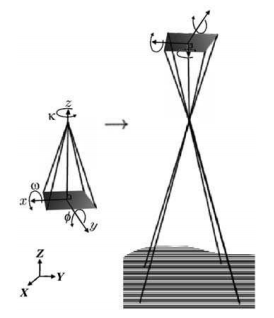
\includegraphics[width=1\hsize]{figuras/atitude.png}
  %\legend{Texto da legenda quando necessário.}
  \source{\cite{coelho2007fotogrametria}}
\end{figure}

Assim,

$\phi$, $\omega$, $\kappa$: Ângulos de Euler, chamados de ângulos de atitude;

$X0$, $Y0$ e $Z0$: Coordenadas no espaço-objeto para o CP da tomada da foto.

O ângulo $\phi$ que corresponde a rotação em relação ao eixo Y, o ângulo $\omega$ que corresponde a rotação em relação ao eixo X e o ângulo $\kappa$ que corresponde a rotação em relação ao eixo Z. Os ângulos de atitude para cada foto registram a angulação de inclinação do avião na hora da tomada da foto.

Uma vez realizada a orientação interior e exterior de uma imagem é possível a obtenção das coordenadas tridimensionais de um ponto na imagem em sua posição correspondente no terreno. A presença dos valores de seus parâmetros caracteriza a etapa de inicialização do processo fotogramétrico como concluída. Assim decidiu-se registrar no modelo de banco a presença dos modelos paramétricos adotados pelas orientações, interior e exterior, bem como seus parâmetros e coeficientes computados por projeto. Os procedimentos e seus parâmetros podem ser armazenados nas classes \textit{Mod\_param}, \textit{Parameter}, \textit{Coef\_img} e \textit{Processing\_metho}.

\begin{description}[labelwidth=2cm, itemsep=-0.3cm]
\item [Classe Mod\_param]
\item[Id:] Índice numérico;
\item[Type:]  Tipo de de operação realizada.
\item[Num\_par:] Quantidade de parâmetros de interesse;
\item[Name:] Nome da operação;
\item[Formula:] Equação e/ou modelo matemático utilizado para o cálculo da operação.
\end{description}

Para que a classe \textit{Mod\_param} se comunique melhor com a classe  \textit{parameter} foi criado o \textit{data type} \textit{type\_op} (figura \ref{top} nos apêndices), onde o tipo de procedimento realizado é previsto.

\begin{description}[labelwidth=2cm, itemsep=-0.3cm]
\item [Classe Parameter]
\item[Id:] Índice numérico;
\item[Sequential:] Número de um ordem sequencial estabelecida para o parâmetro;
\item[Name:] Nome do parâmetro;
\item[Symbol:] Simbolo que represente o parâmetro;
\item[Id\_mpar:] Referência para a classe \textit{Mod\_param}.
\end{description}

\begin{description}[labelwidth=2cm, itemsep=-0.3cm]
\item [Classe Coef\_img]
\item[Id:] Índice numérico;
\item[Id\_img:] Referência para a classe `Image’;
\item[Id\_proj:] Referência para a classe `Project';
\item[Value:] Valor do coeficiente gerado; 
\item[Id\_pmet:]  Referência para a classe `Processing\_metho'.
\end{description}

\begin{description}[labelwidth=2cm, itemsep=-0.3cm]
\item [Classe Processing\_method]
\item[Id:] Índice numérico;
\item[Data\_origin:] Tipo de procedimento q gera o coeficiente.
\end{description}

Os parâmetros da orientação exterior de uma imagem podem ser fornecidos por intermédio de sistemas auxiliares, tais como GNSS, para o cálculo das coordenadas do CP, e pelos Sistemas de Navegação e medição inerciais, situação na qual são fornecidos os ângulos de atitude do sensor no instante de cada tomada fotográfica. Para o primeiro caso foi criada a classe \textit{frame\_gnss}, para o segundo, \textit{frame\_ins}. Ambas as classes possuem um atributo booleano chamado `status'. Se o mesmo for nulo assumi-se que estes valores são desconhecidos e logo a tupla não existirá. Se este valor for verdadeiro, então tem-se que os dados são `fixos'. Se o valor for falso entende-se que esses valores são `iniciais'.

\begin{description}[labelwidth=2cm, itemsep=-0.3cm]
\item [Classe Frame\_gnss]
\item[Id:] Índice numérico;
\item[Status:] Indicador booleano do status dos dados de entrada;
\item[Geom:] Coordenadas de entrada do CP da imagem;
\item[Sigma\_E:] Desvio-padrão da coordenada E;
\item[Sigma\_N:] Desvio-padrão da coordenada N;
\item[Sigma\_H:] Desvio-padrão da coordenada H;
\end{description}

\begin{description}[labelwidth=2cm, itemsep=-0.3cm]
\item [Classe Frame\_ins]
\item[Id:] Índice numérico;
\item[Status:] Indicador booleano do status dos dados de entrada;
\item[Omega:] Ângulo de atitude $\omega$ de entrada da imagem;
\item[Phi:] Ângulo de atitude $\phi$ de entrada da imagem;
\item[Kappa:] Ângulo de atitude $\kappa$ de entrada da imagem;
\item[S\_omega:] Desvio-padrão do angulo $\omega$;
\item[S\_phi:] Desvio-padrão do angulo $\phi$;
\item[S\_kappa:] Desvio-padrão do angulo $\kappa$;
\end{description}

A figura \ref{pack_img} apresenta como estas classes interagem se comunicam.

\begin{landscape}
\begin{figure}[ht]{23cm}
  \caption{Pacote Image.} \label{pack_img}
  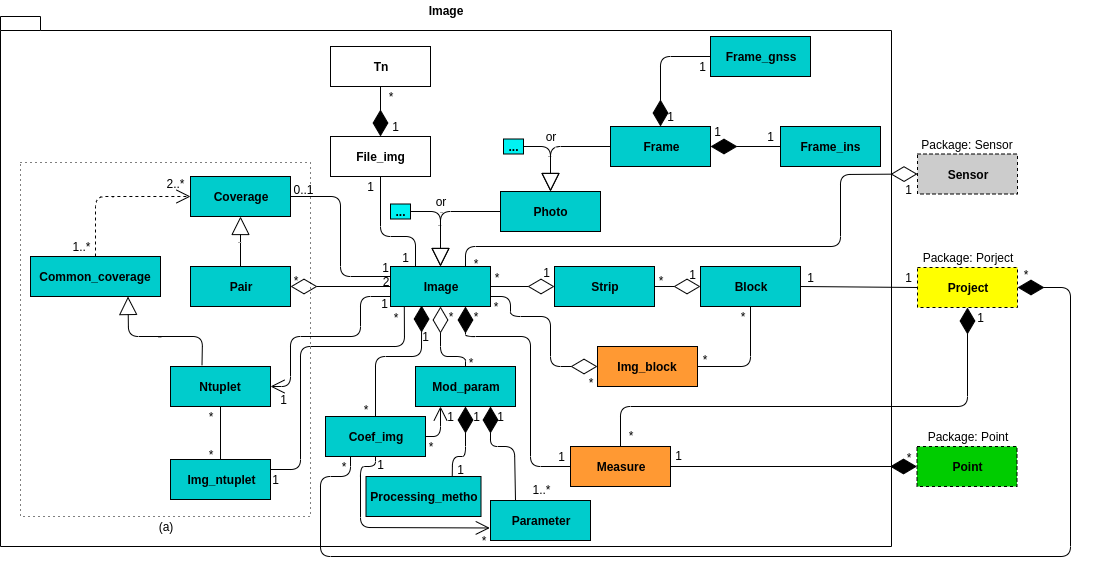
\includegraphics[width=\hsize]{figuras/package_img.png}
  \legend{(a) conjunto de classes que podem se tornar um sub-pacote.}
  \source{A autora, 2019}
\end{figure}
\end{landscape}

%Essa subseção gera em anexo modelos, LEMBRAR: de disponibilizar também o arquivo digital, não somente a imagem impressa (deixando isso bem claro no trabalho)
Não se entrou em detalhes quanto ao produtos finais de um projeto fotogramétrico. Isso se dá pelo fato de que para o pacote produto a variedade de variáveis e possíveis produtos é tão complexa que se optou neste trabalho por não mapeá-los no modelo. Vale ressaltar que em alguns momentos o modelo deixa indicado onde possíveis extensões podem ocorrer, inclusive os produtos ortofoto e por consequência ortomosaico. Porém deve ser deixar claro que nenhum produto final é contemplado no modelo conceitual. A extensão do mesmo com a inclusão do pacote de produtos é um possível futuro trabalho a ser realizado.

O modelo com todas classes e suas conexões detalhado é grande e complexo, de modo que foi optado por não inseri-lo no texto. O mesmo se encontra apresentado na figura \ref{modelo_00} no apêndice \ref{ap-1}. Um arquivo digital da imagem deste modelo será disponibilizado para que assim seja possível uma leitura do modelo como um todo.

Desde a primeira versão até a versão final apresentada neste texto, o modelo orientado a a objeto sofreu diversas modificações. Três meses após o início da modelagem percebeu-se que o método de processo de desenvolvimento monolítico, até então utilizado, corria o risco de não se cumprir o prazo estabelecido. Isso acarretou na transição para o método de processo de desenvolvimento ágil. Até aquele momento o modelo havia sido trabalhado com apoio da fundamentação teórica. A partir daquele momento, houve a preocupação da geração de um código base, implementação de um banco de dados usando esse código e a realização de testes que verificassem a integridade técnica do banco. 

O código base, do qual se implementaria um banco de dados baseado neste modelo deveria ser gerado automaticamente pela ferramenta utilizada para desenhar o mesmo. A ferramenta escolhida foi o Umbrello. Isso aconteceu pois a ferramenta em questão atende a linguagem UML 2.0, e e capaz de gerar um código em sql a partir do modelo desenhado. Outras ferramentas no mercado, de conhecimento da autora, são pagas ou não comportam as necessidades do modelo devido sua complexidade. Dentre essas ferramentas, existem plataformas que trabalham com as linguagens de Geoframe e OMT-G, o que implicou na escolha da linguagem UML 2.0. O problema encontrado foi que o sql gerado a partir do modelo desenhado possui uma quantidade de erros e inconsistências considerada demasiadamente alta, o que tornava o código inviável para utilização. A solução pensada foi a tradução do modelo até então trabalhado para um modelo relacional. Dessa forma, agora num processo ágil, toda mudança realizada no código por causa de testes, agora afetava o modelo relacional e o modelo orientado a objeto.


\subsection{Modelo Relacional}

Apesar do que foi citado no item \ref{sgbdr}, a despeito do que informa Korth, foi necessária adaptação de parte da modelagem OO realizada para um Modelo Relacional. Utilizando a ferramenta online ERDplus, adaptações foram realizadas. Heranças do modelo orientado objeto viraram \textit{constrains} sequenciais de FK no modelo relacional. Os dados complexos que até o momento tinham tipos específicos, viraram tipos alfanuméricos. Modificações no código então se fizeram necessárias. Essa modificações só foram possíveis pois já que o banco seria codificado como relacional, optou-se por escolher um banco que possuísse uma extensão geográfica. Assim gerando um código base que implementasse um banco objeto relacional.

Devido a seus tamanho junto ao fato de que todas as suas classes foram apresentadas anteriormente, optou-se por não colocar o modelo no texto deste documento. Porém o mesmo encontra-se na figura \ref{modelo_r} do apêndice \ref{ap-1}.

O modelo relacional foi usado como um `gap' que permitisse a geração do código de forma a otimizar o tempo disponível. A utilização do mesmo resultou na implementação de um banco de dados objeto relacional.



\section{Implementação do Projeto Piloto}

O software aplicativo de banco de dados escolhido para a implementação do modelo foi o PostgreSQL. Devido à sua capacidade de armazenar e manipular dados geográficos, utiliza-se também da extensão PostGIS. Todas as classes de estereótipo de dados geográfico apresentadas no modelo, \textbf{point}, \textbf{polygon} e \textbf{raster}, precisaram utilizar em sua programação e carga comandos específicos. Este só foram possíveis pela utilização da extensão espacial no banco. A figura \ref{postpost} ilustra esta integração.

\begin{figure}[!ht]{10cm}
  \caption{Integração PostgreSQL e Postgis} \label{postpost}
  \centering
  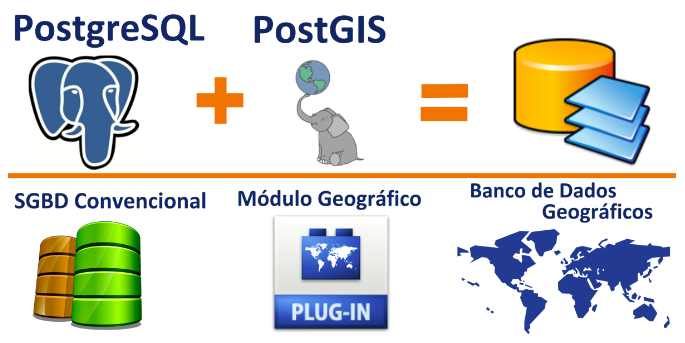
\includegraphics[width=1\hsize]{figuras/postgre_postgis.png}
  %\legend{Texto da legenda quando necessário.}
  \source{\cite{clickgeosgbd}}
\end{figure}

A codificação de criação das estruturas do banco não necessariamente precisa de uma interface. Por questões de familiaridade da autora com a plataforma optou-se por fazer a implementação do mesmo por uma interface de administração do SGBD. A interface escolhida foi o PgAdmin III.

A grande maioria dos testes de verificação e validação realizados neste trabalho foram feitos por processos de \textit{query} usando a linguagem sql. A `query' pode ser entendida como pedido, consulta, solicitação ou requisição de informações ou dados presentes num banco, utilizando um código pré-definido. Neste caso o código é o sql, como previamente comentado.

O código de geração das tabelas e tipos de dados do projeto piloto se encontra no apêndice \ref{ap1}. Este contém 446 linhas, compostas de códigos e comentários feitos em sql. O código foi feito em cascata, com exceção de uma pequena parte ao final desse código. Dessa forma, basicamente todas as tabelas presentes no banco são criadas em conjunto a criação de seu esquema. Isso resulta que ao utilizar o código disponível neste documento, a criação do banco é realizada quase que de uma só vez. Faltando somente a criação das tabelas responsáveis pelo armazenamento das fotografias no banco de dados. Este caso particular será apresentado ao final da próxima seção. 



\section{Carga}\label{cargs}

Com o código base gerado, o tipo de banco escolhido e as modificações necessárias para que esse código pudesse armazenar os dados geográficos no banco, o próximo passo foi a implementação do banco de dados piloto.

Como o código inicial era extenso, o mesmo foi `quebrado' à medida que foi testado e implementado. Cada tabela foi testada sozinha, de forma a verificar a sintaxe do código. Quando uma tabela passava no teste, a seguinte era acoplada ao código trabalhado. O novo segmento de código, agora contando as partes verificadas e uma tabela não testada era testado novamente, verificado, e corrigido se necessário. Esse processo era repetido até que o novo código passasse pelo teste e pudesse ser adicionado à uma nova parte do código base.  Assim entrou-se num processo em loop de testes, correções e acréscimos ao código que em muito se assemelha ao processo TDD, explicado no item \ref{proc}. A principal diferença é que um processo TDD é desde seu início um processo ágil, enquanto este trabalho começou como um processo monolítico, antes de migrar para o processo ágil. Assim não se pode dizer que o trabalho siga o modelo TDD, e sim que se aproxima do mesmo. Toda correção que não fosse de sintaxe, gerava alterações nos modelos, tanto no relacional quanto no orientado a objeto. Assim, houve uma correção constante de ambos os modelos, de forma a não se perder detalhes do processo. Ao final, o banco gerado foi apagado para que numa última bateria de testes do código fosse implementada por inteiro. Essa fase de implementação e testes foi, o que se pode entender como a primeira fase de verificação. A partir deste momento tinha-se um banco implementado e aparentemente verificado. Novamente realizando testes, começou-se a realizar 'cargas' por cada tabela no banco. Iniciou-se então um novo loop. Agora o objetivo não era só saber se o banco funcionava, mas sim se ele suportava os dados fornecidos pelo LFSR. Entra-se então na segunda fase de verificação com testes, erros, correções e incrementos do código. A diferença é que nesta segunda bateria de testes, a expectativa era de uma quantidade menor de erros. Em compensação, grande parte dos erros descobertos e corrigidos ao realizar essas cargas geravam modificações no código-base trabalhado, nos modelos e testes do próprio código. Um exemplo do exposto é a classe \textit{measure}, onde inicialmente não continha o atributo `Id\_proj', este por sua vez relaciona a medida do ponto na imagem à um projeto, assim evitando que medições de um mesmo ponto em uma mesma imagem se confundissem.

Todas as cargas foram feitas por meio de `querys', com exceção das necessárias para os arquivos ``raster'' das imagens. O código abaixo é exemplo de uma carga de dados alfanuméricos (parte do código presente no apêndice \ref{carga1}).

\begin{lstlisting}
INSERT INTO efoto.Fiducials (Id,x,y,Sigma_x,Sigma_y,Id_calib)
VALUES
('1','113','0.016',null, null,'1'),
('2','-113.006','0.018',null, null,'1'),
('3','0.004','113.015',null, null,'1'),
('4','0.007','-112.975',null, null,'1');
\end{lstlisting}

Nesta carga, foram armazenados na tabela `Fiducials' os valores das coordenadas das marcas fiduciais. Estes foram obtidos no certificado de calibração do sensor já armazenado no banco. Outro exemplo de carga é o realizado na tabela de pontos. 

O exemplo a seguir é parte de uma das cargas realizadas (o código da carga completa se encontra no apêndice \ref{carga2}).

\begin{lstlisting}
INSERT INTO efoto.Point (Id, Name_, Geom, Sigma, Id_coll)
VALUES
('14','LH1',ST_Transform(ST_GeomFromText('POINTZ(680947.997 7464833.669 3.942)',32723),4326),null,'7'),
('15','LH2',ST_Transform(ST_GeomFromText('POINTZ(680895.378 7463828.578 9.206)',32723),4326),null,'7'),
('16','LH3',ST_Transform(ST_GeomFromText('POINTZ(682227.162 7464200.581 2.184)',32723),4326),null,'7');
\end{lstlisting}

Diferentemente do primeiro exemplo, esta segunda carga possui dados complexos. Neste caso refere-se às coordenadas geográficas dos pontos armazenados.  Estes só puderam ser armazenados devido o uso da extensão Postgis. Para isto, foi utilizado o domínio `POINTZ', que permite o armazenamento de coordenadas 3D para pontos padronizado como um dado geográfico, que usa o EPSG:4326, ou seja, possui como sistema de referência geodésico o WSG 84. A principal diferença entre dados geográficos para dados geométricos para o Postgis é que o primeiro assume que os dados carregados são compostos por pontos na superfície da Terra, enquanto para os dados ditos geométricos se assume que estes dados se encontram num plano plano cartesiano, como uma projeção cartográfica. 
Como visto no exemplo, as coordenadas de entrada estão na projeção UTM, isso significa que devem ocorrer algumas transformações ao armazenar esses dados. Usando a função ``ST\_GeomFromText()'', é contruído um objeto geométrico baseado no WKT (well-know text) e no SRS (spacial reference system) de origem. A partir desse ponto é feita a conversão deste dado para o SRS do banco com a função ``ST\_Transform()''. O segmento do exemplo anterior, mostrado a seguir, possui as transformações explicadas:

\begin{verbatim}
    ST_Transform(ST_GeomFromText('POINTZ(680947.997
    7464833.669 3.942)',32723)
\end{verbatim}

Qualquer que seja o valor dos dados geográficos a ser armazenado em um banco de dados, deve-se considerar suas projeções e sistemas de referência. Logo, deve-se ter conhecimento de quais valores do índice do EPSG, e se necessário, quais transformações serão necessários para a realização do armazenamento correto de tais dados.

Foram realizadas 3 cargas de grupos de dados. A primeira consistindo dos dados do projetos `UERJ-OI',`UERJ-OI-OE' e `UER-no-orient' disponíveis pela plataforma E-foto em sua webpage (http://www.efoto.eng.uerj.br/). A segunda carga foi disponibilizada pelo LFSR como parte do material do projeto `Análise comparativa do potencial das medições estereoscópicas dos sensores ULTRACAM e WORLDVIEW' do aluno Luiz Henrique de C. Freires. Ambas as cargas possuíam dados alfanuméricos e geográficos. Porém, devido à uma particularidade dos dados raster, as imagens foram armazenadas no banco por uso do terminal de comando do computador local do banco, ao invés de usar a interface PgAdmin3. Isso implicou em uma terceira carga.

Enquanto na teoria é fato de que é possível armazenar arquivos do tipo raster em um banco de dados, a realidade é que os meios para se realizar tal ação são poucos, e muitas vezes, difíceis de se utilizar. A ferramenta de linha de comando `raster2pgsql' é compilada dentro do Postgis, e preferida para o armazenamento de dados raster por muitos usuários do Postgis. Os tipos de arquivos raster que esta ferramenta suporta são, em sua maioria, compatíveis com a Geospatial Data Abstraction Library - GDAL, que é uma biblioteca computacional para leitura e criação de dados de cunho espacial: vetoriais e matriciais.
Devido a este fato decidiu-se realizar o armazenamento das imagens utilizando `raster2pgsql' pelo terminal de comando da máquina local do banco de dados.

Este processo seguiu duas etapas principais. A geração de um arquivo '.sql' a partir do arquivo raster de interesse, e o armazenamento do mesmo no banco de dados. Em uma visão geral, a linha de comando para criação do `.sql' se apresenta da seguinte forma:

\begin{verbatim}
    raster2pgsql <comandos específicos> <imagem> schema.tabela 
    > caminho do arquivo a ser gerado/arquivo.sql
\end{verbatim}

Este mesmo comando foi utilizado para gerar os arquivos importados posteriormente para o banco, tal como visto no exemplo a seguir:

\begin{verbatim}
    raster2pgsql -t "auto" -c -M
    /home/tatyana/bd/efoto/1997_016_300dpi.bmp
    img.t1 > /home/tatyana/bd/imgsbd/t1.sql
\end{verbatim}

Com o arquivo gerado, o mesmo pôde ser carregado no banco. Para o `.sql' do exemplo anterior foi realizado o seguinte comando:

\begin{verbatim}
/home/tatyana/bd/imgsbd$ psql -d teste -f t1.sql    
\end{verbatim}

Devido ao tamanho do arquivo de uma imagem e as limitações da máquina onde se encontra o banco de dados teste, optou-se pelo armazenamento das imagens fornecidas pelo projeto E-Foto. Há de ser notado, que neste caso particular, como foram poucas as imagens armazenadas no banco, cada imagem foi carregada manualmente de forma singular. Porém existem casos onde o usuário pretende importar uma grande quantidade de imagens para o banco. Nestes casos os chamados para o raster2pgsql podem ser inclusos num script que administre o processo, como o script\footnote{Codificado e cedido pelo Professor Irving Badolato especificamente para servir de apoio aos testes deste trabalho.} desenvolvido em python e apresentado no anexo \ref{script1}.

Continuando a analisar o último comando, tem-se que este não só carrega uma imagem, ele também cria a tabela onde essa imagem deverá ser armazenada. O Postgis, diferentemente de outros bancos de dados, adota a visão de um raster para uma tabela. Nessa estrutura de dados não existe uma tabela para o dado e outra para o metadado. O que se tem é um atributo do tipo raster que armazena o próprio dado e suas informações geoespaciais. Com este comando de criação e importação para o banco de dados do arquivo, é adotado por padrão a composição da tabela destinatária pelos atributos: `rid' como o índice numérico, e `ras' com o tipo de dado raster. Assim, prezando a coerência e a fluência dos dados, foi criado outro \textit{schema} exclusivo para as imagens. Desta forma, cada tabela desse \textit{schema} é um arquivo raster. As imagens podem ser carregadas dentro deste, dentro de vários \textit{schemas} ou até mesmo num servidor separado, contanto que seu nome e local estejam informados no banco, como previsto na classe `File\_img', e que o banco possa se conectar a esse local. Assim o usuário terá total acesso ao arquivo que o LFSR disponibilize para trabalho.

Existe um conjunto de tabelas modeladas para o banco, que atualmente não possuem dados. São as tabelas de geração e armazenamento de um rodapé de imagem. Este rodapé pode ser gerado a partir da programação de um gatilho no banco; Porém, devido à falta de dados e tempo necessário para realizar tal processo, deixa-se indicado a criação desta função como uma extensão para o banco de dados do LFSR. 
A partir do momento em que todos os dados disponibilizados foram carregados no banco pode se afirmar que o banco está operacional.

\section{Consultas}

Continuando o fluxo de processos, a etapa seguinte constituiu na elaboração de consultas que retornassem os dados levantados como requisitos apresentados no capítulo \ref{met}. Para tanto, foi realizado um novo brainstorm onde o professor da disciplina de fotogrametria foi questionado sobre quais tipos de perguntas ele esperava que um banco de dados do LFSR fosse capaz de responder.

Estas perguntas geraram os códigos presentes no apêndice \ref{crg} que, por sua vez, se apresentam no formato de consultas em sql. A capacidade de responder a essas consultas foi verificado por intermédio da realização de testes que validam o banco de dados piloto.

Essas consultas, acrescidas de seus resultados, serão apresentadas no capítulo \ref{carga}.

\section{Teste Final}\label{testefinal}

Por fim, a geração da documentação técnica do banco de dados desenvolvido neste trabalho permitiu a sua réplica em um dos computadores do LFSR. Nesse sentido foi realizado um último teste, consistindo no espelhamento da implementação do banco de dados dentro de uma outra máquina. Este teste foi concluído com sucesso. O código-fonte resultante da implementação encontra-se disponível no apêndice \ref{cdg}.


